\documentclass[a4paper]{article}
\usepackage{amsmath,amssymb,caption,float,graphicx,hyperref,indentfirst,minted,multirow,tabularx,xcolor}
\usepackage[utf8]{inputenc}
\usepackage[english]{babel}
\usepackage[backend=bibtex]{biblatex}
\addbibresource{Lab4.bib}
\captionsetup[figure]{labelsep=period}
\captionsetup[table]{labelsep=period}
\definecolor{bg}{rgb}{0.95,0.95,0.95}
% \hypersetup{
%     colorlinks=true,
%     linkcolor=blue,
%     filecolor=magenta,      
%     urlcolor=cyan,
% }
\renewcommand\thesection{\arabic{section}}
\usemintedstyle{emacs}
\begin{document}
\begin{center}
    \huge
    \textbf{VE482\\Introduction to Operating Systems\\}
    \Large
    \vspace{15pt}
    \uppercase{\textbf{Lab 4}}\\
    \large
    \vspace{5pt}\today\\
    \vspace{5pt}
    Yihua Liu 518021910998
    \vspace{5pt}
    \rule[-5pt]{.97\linewidth}{0.05em}
\end{center}
\section{Database}
This is the evening, you are exhausted after a long day of work on \texttt{mumsh}, so you decide to poke around and learn more about database, as unfortunately you never had an opportunity to select such course during your studies.
\subsection{Database creation}
\begin{minted}[frame=single,bgcolor=bg,breaklines]{bash}
git log --pretty="%H,%aN,%aI,%s" > db.csv
\end{minted}
\begin{figure}[H]
    \centering
    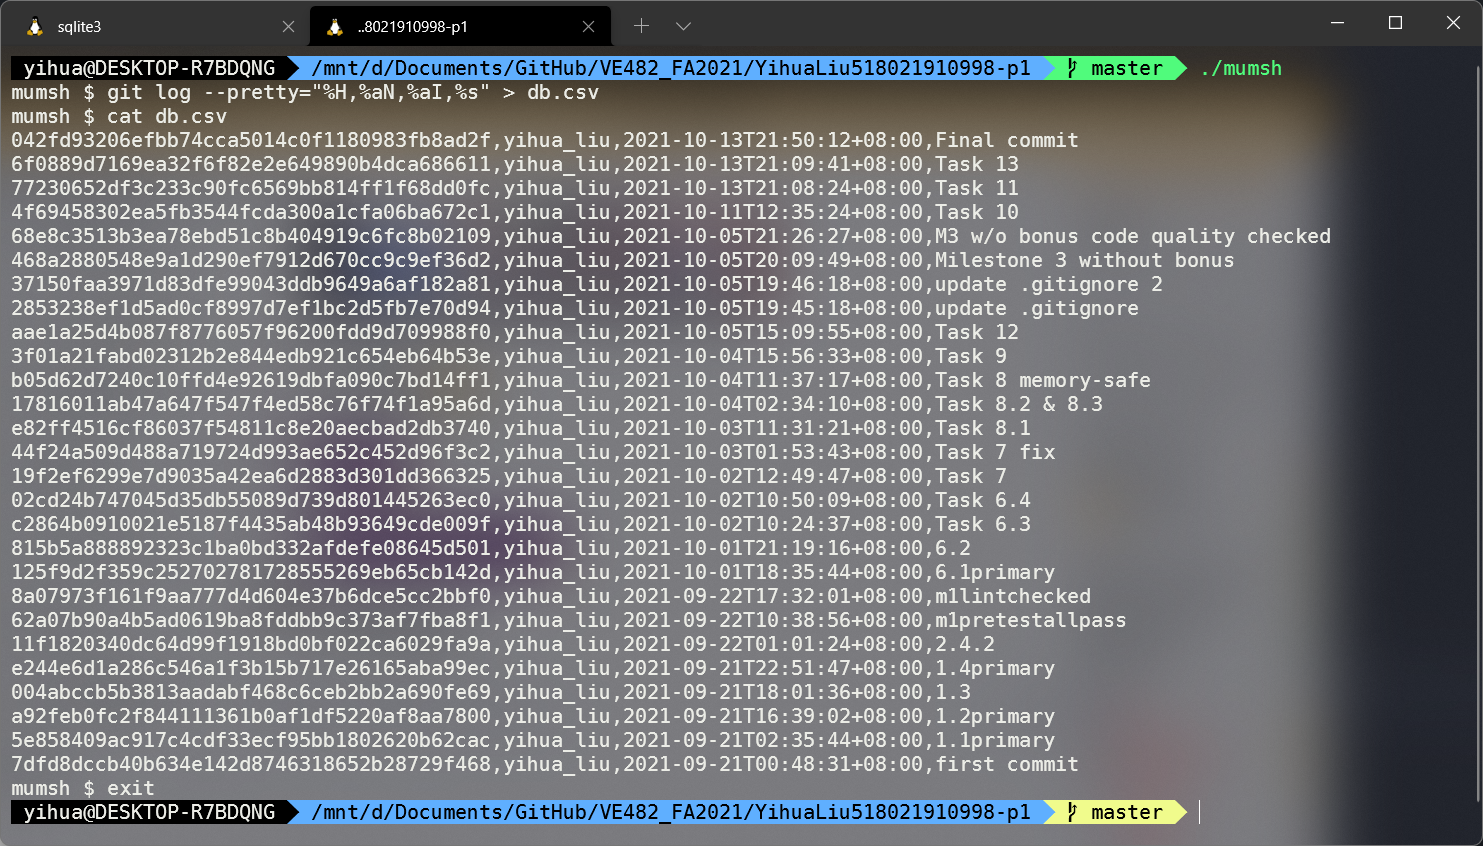
\includegraphics[width=1\textwidth]{1.png}
    \caption{Test database generation.}
\end{figure}
\begin{figure}[H]
    \centering
    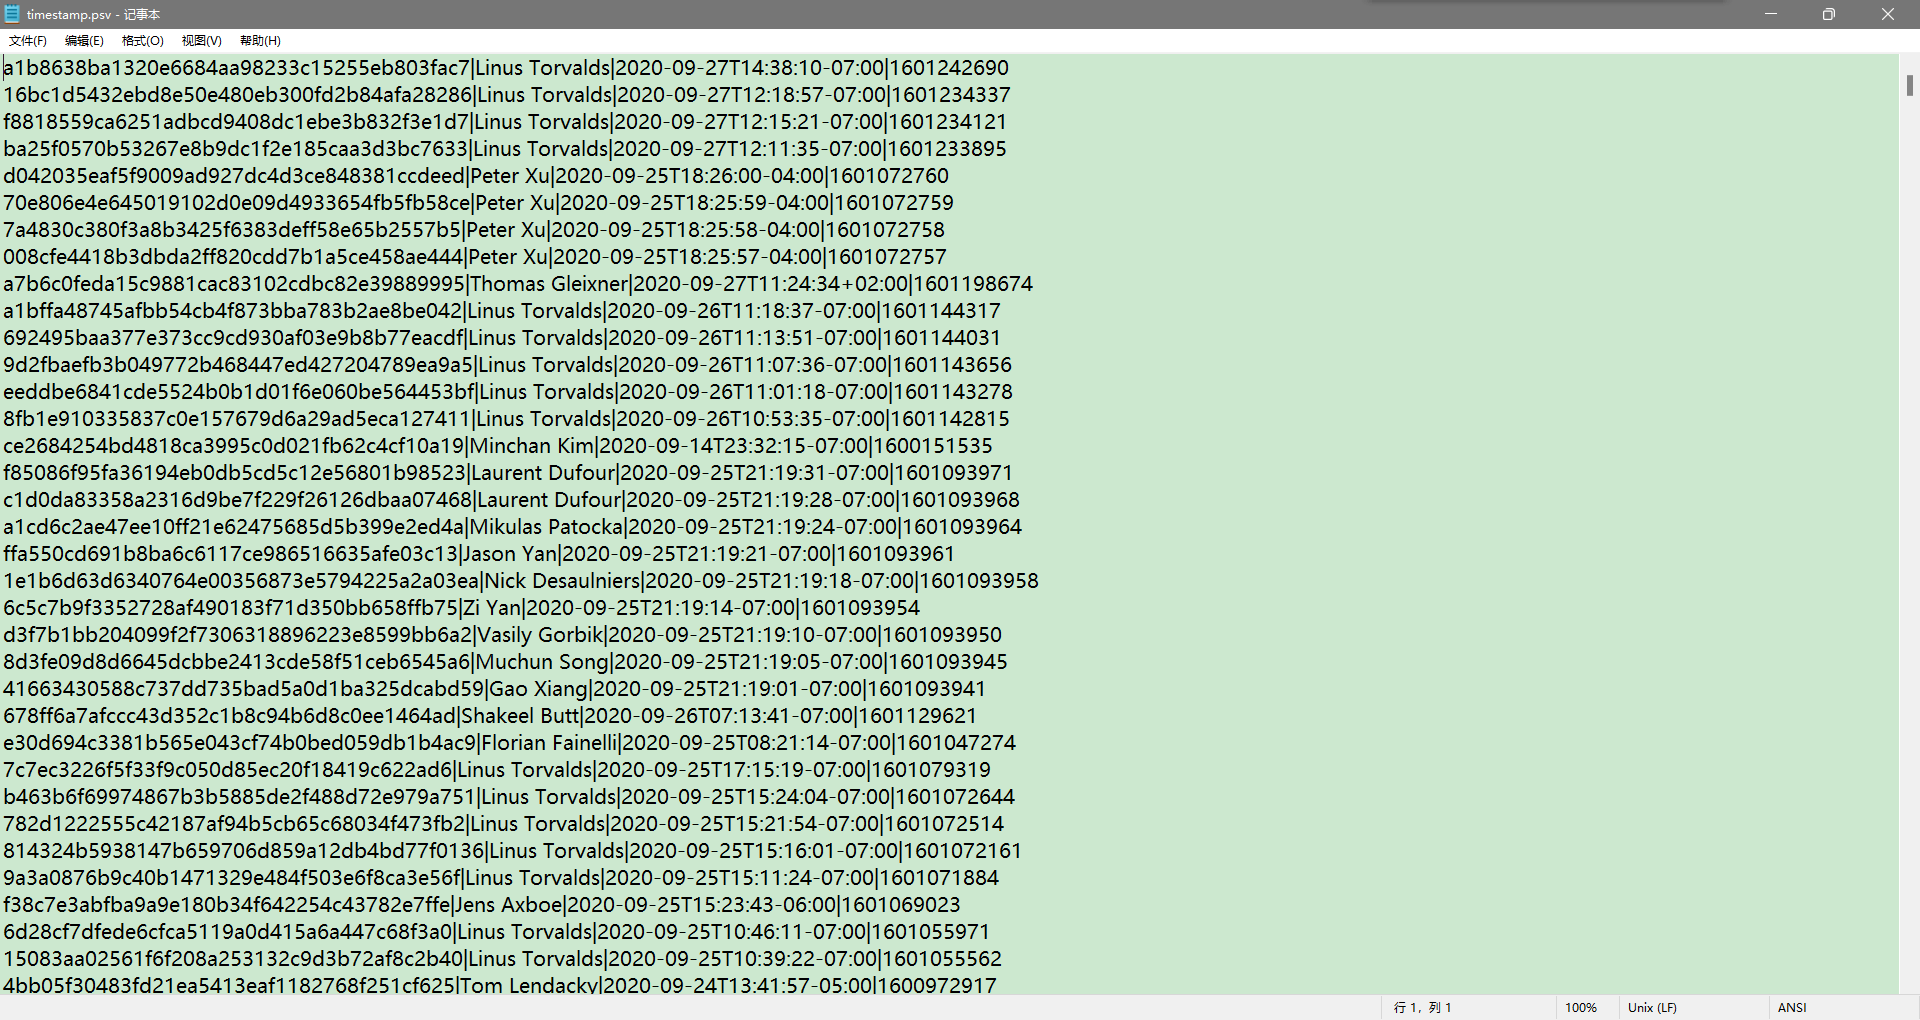
\includegraphics[width=1\textwidth]{2.png}
    \caption{Fields for \texttt{timestamp.psv}.}
\end{figure}
\begin{figure}[H]
    \centering
    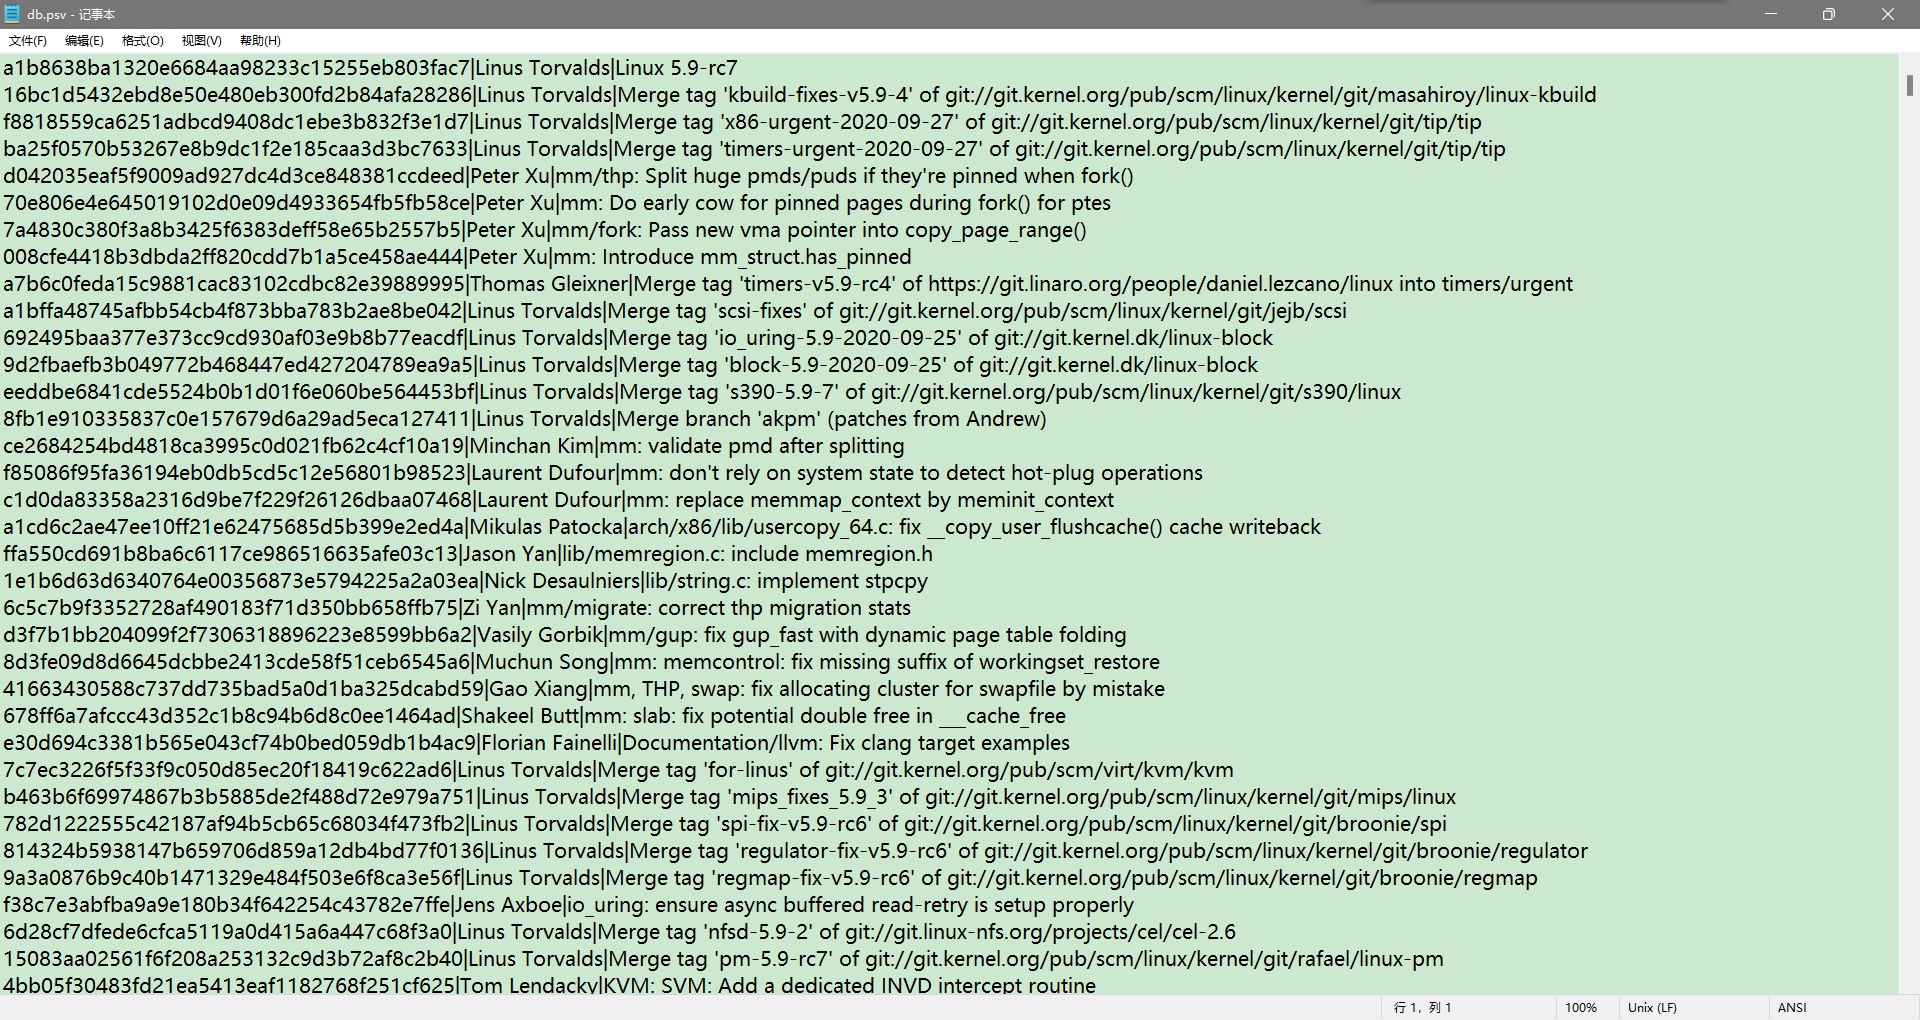
\includegraphics[width=1\textwidth]{3.png}
    \caption{Fields for \texttt{db.psv}.}
\end{figure}
We use \texttt{db.psv} and \texttt{timestamp.psv} provided by TAs on Canvas instead of \texttt{db.csv} and \texttt{timestamp.csv} because we cannot find them on the server in the directory \texttt{ve482/14}.
\subsection{Database system installation}
As you want to ensure your understanding and guesses are correct you need to verify a few things online. Luckily your VPN is now working, so you can use a proper search engine and ensure the correctness of what you found.
\begin{itemize}
    \item What are the most common database systems?\\
    Oracle, MySQL, Microsoft SQL Server, MongoDB, Redis, SQLite, Microsoft Access, etc.
    \item Briefly list the pros and cons of the three most common ones.\\
    \begin{table}[H]
        \centering
        \begin{tabular}{|c|c|c|}
            % \hline
            % Name&Pros&Cons\\
            \hline
            \multirow{2}{*}{Oracle}&Pros&Robust, strong and abundant features, state-of-the-art\\
            \cline{2-3}
            &Cons&Expensive, occupying much resources\\
            \hline
            \multirow{2}{*}{MySQL}&Pros&Available for free, extensible, high-customization\\
            \cline{2-3}
            &Cons&Complex to use, some features are missing\\
            \hline
            Microsoft&Pros&Robust, strong and abundant features, fast and stable\\
            \cline{2-3}
            SQL Server&Cons&Very expensive, occupying much resources\\
            \hline
        \end{tabular}
        \caption{The pros and cons of the three most common database systems \cite{dbsys}.}
    \end{table}
\end{itemize}
After completing your reading you decide to install \texttt{SQLite} on your Linux system. The next step is now to import your git database into two tables.
\begin{itemize}
    \item Create an empty SQLite database.
    \begin{minted}[frame=single,bgcolor=bg,breaklines]{bash}
sudo apt install sqlite3
sqlite3 l4.db
    \end{minted}
    \begin{figure}[H]
        \centering
        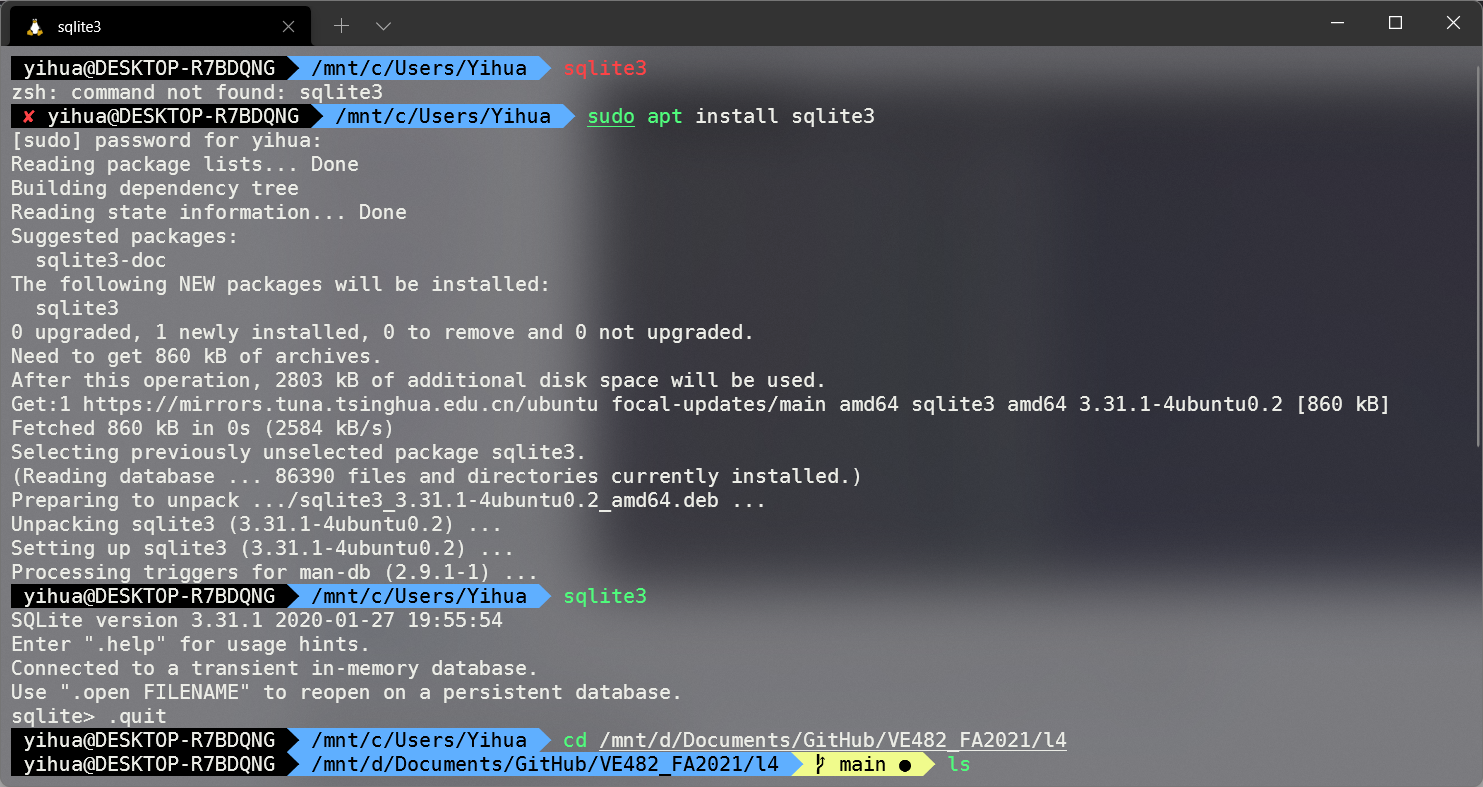
\includegraphics[width=1\textwidth]{4.png}
        \caption{Create an empty SQLite database.}
    \end{figure}
    \item Use the SQLite shell to prepare two empty tables for each of your .csv file.
    \begin{minted}[frame=single,bgcolor=bg,breaklines]{sql}
CREATE TABLE db
(
    hash TEXT NOT NULL,
    name TEXT NOT NULL,
    comment TEXT NOT NULL
);
CREATE TABLE time_stamp
(
    hash TEXT NOT NULL,
    name TEXT NOT NULL,
    dates TEXT,
    tstamp INT
);
    \end{minted}
    \begin{figure}[H]
        \centering
        
\includegraphics[width=1\textwidth]{5.png}
        \caption{Use the SQLite shell to prepare two empty tables for each of your .csv file.}
    \end{figure}
    \item Import each .csv file in its corresponding SQLite table.
    \begin{minted}[frame=single,bgcolor=bg,breaklines]{sql}
.separator "|"
.import db.psv db
.import timestamp.psv time_stamp
    \end{minted}
    \begin{figure}[H]
        \centering
        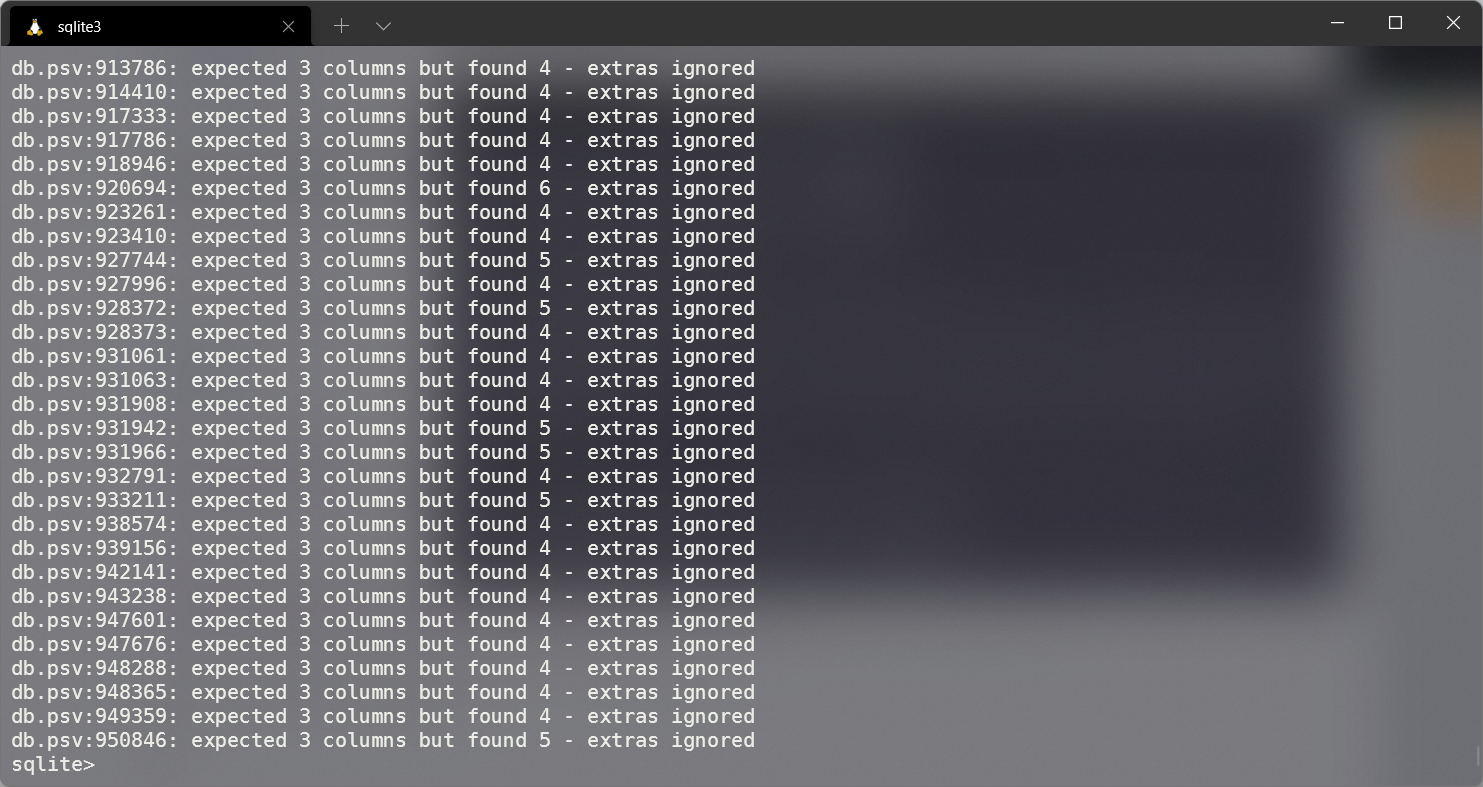
\includegraphics[width=1\textwidth]{6.png}
        \caption{Import db.psv in its corresponding SQLite table.}
    \end{figure}
    \begin{figure}[H]
        \centering
        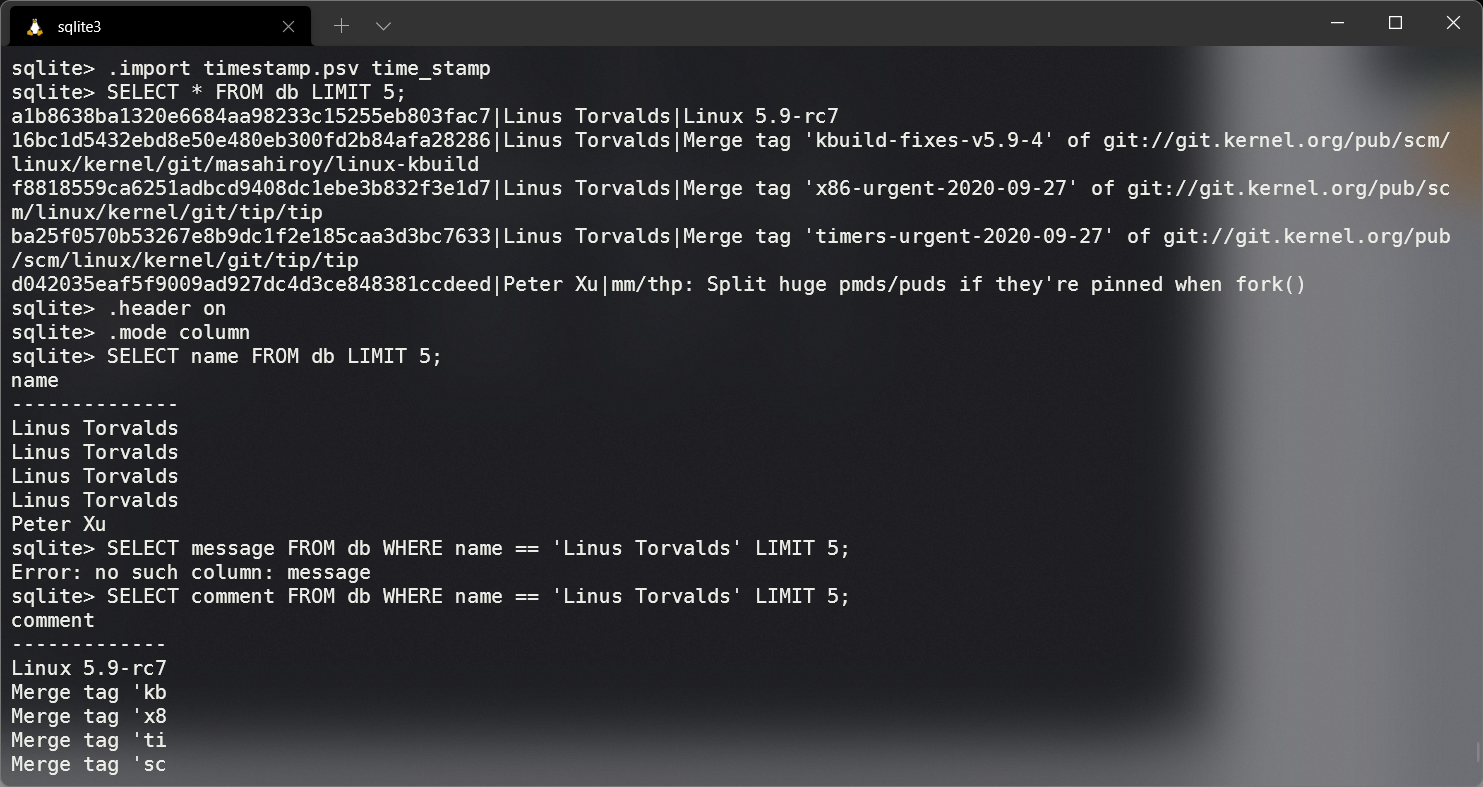
\includegraphics[width=1\textwidth]{7.png}
        \caption{Import timestamp.psv in its corresponding SQLite table.}
    \end{figure}
\end{itemize}
\subsection{Database queries}
At this stage you want to run basic queries to verify that the database has been imported correctly. Therefore you spend the rest of the evening playing around the database and running queries.
\begin{itemize}
    \item Who are the top five contributors to the Linux kernel since the beginning?\\
    \begin{minted}[frame=single,bgcolor=bg,breaklines]{sql}
SELECT name, COUNT(name) FROM time_stamp GROUP BY name ORDER BY COUNT(name) DESC LIMIT 5;
    \end{minted}
    \begin{minted}[frame=single,bgcolor=bg,breaklines]{text}
Linus Torvalds|30702
David S. Miller|13180
Takashi Iwai|7726
Mark Brown|7670
Arnd Bergmann|7520
    \end{minted}
    \item Who are the top five contributors to the Linux kernel for each year over the past five years?
    \begin{minted}[frame=single,bgcolor=bg,breaklines]{sql}
SELECT name, COUNT(name) FROM time_stamp WHERE dates BETWEEN DATETIME('now','-5 year') AND DATETIME('now','-4 year') GROUP BY name ORDER BY COUNT(name) DESC LIMIT 5;
SELECT name, COUNT(name) FROM time_stamp WHERE dates BETWEEN DATETIME('now','-4 year') AND DATETIME('now','-3 year') GROUP BY name ORDER BY COUNT(name) DESC LIMIT 5;
SELECT name, COUNT(name) FROM time_stamp WHERE dates BETWEEN DATETIME('now','-3 year') AND DATETIME('now','-2 year') GROUP BY name ORDER BY COUNT(name) DESC LIMIT 5;
SELECT name, COUNT(name) FROM time_stamp WHERE dates BETWEEN DATETIME('now','-2 year') AND DATETIME('now','-1 year') GROUP BY name ORDER BY COUNT(name) DESC LIMIT 5;
SELECT name, COUNT(name) FROM time_stamp WHERE dates BETWEEN DATETIME('now','-1 year') AND DATETIME('now') GROUP BY name ORDER BY COUNT(name) DESC LIMIT 5;
    \end{minted}
    From 5 years ago to 4 years ago:
    \begin{minted}[frame=single,bgcolor=bg,breaklines]{text}
Linus Torvalds|2292
David S. Miller|1365
Chris Wilson|1085
Arnd Bergmann|1016
Arvind Yadav|764
    \end{minted}
    From 4 years ago to 3 years ago:
    \begin{minted}[frame=single,bgcolor=bg,breaklines]{text}
Linus Torvalds|2113
David S. Miller|1426
Arnd Bergmann|1147
Colin Ian King|831
Chris Wilson|812
Arvind Yadav|764
    \end{minted}
    From 3 years ago to 2 years ago:
    \begin{minted}[frame=single,bgcolor=bg,breaklines]{text}
Linus Torvalds|2440
David S. Miller|1241
Christoph Hellwig|967
YueHaibing|935
Chris Wilson|910
    \end{minted}
    From 1 years ago to 1 year ago:
    \begin{minted}[frame=single,bgcolor=bg,breaklines]{text}
Linus Torvalds|2358
David S. Miller|1166
Christoph Hellwig|1001
Chris Wilson|985
Mauro Carvalho Chehab|771
    \end{minted}
    From 1 year ago to now:
    \begin{minted}[frame=single,bgcolor=bg,breaklines]{text}

    \end{minted}
    This is empty because the data only records till 2020-09-27T14:38:10-07:00. In MySQL, you can use sentences like \texttt{FROM\_UNIXTIME('tstamp') > DATE\_SUB(NOW(), INTERVAL 5 YEAR)} or \texttt{tstamp > UNIX\_TIMESTAMP(DATE\_SUB(NOW(), INTERVAL 5 YEAR))} \cite{tstamp}.
    \begin{figure}[H]
        \centering
        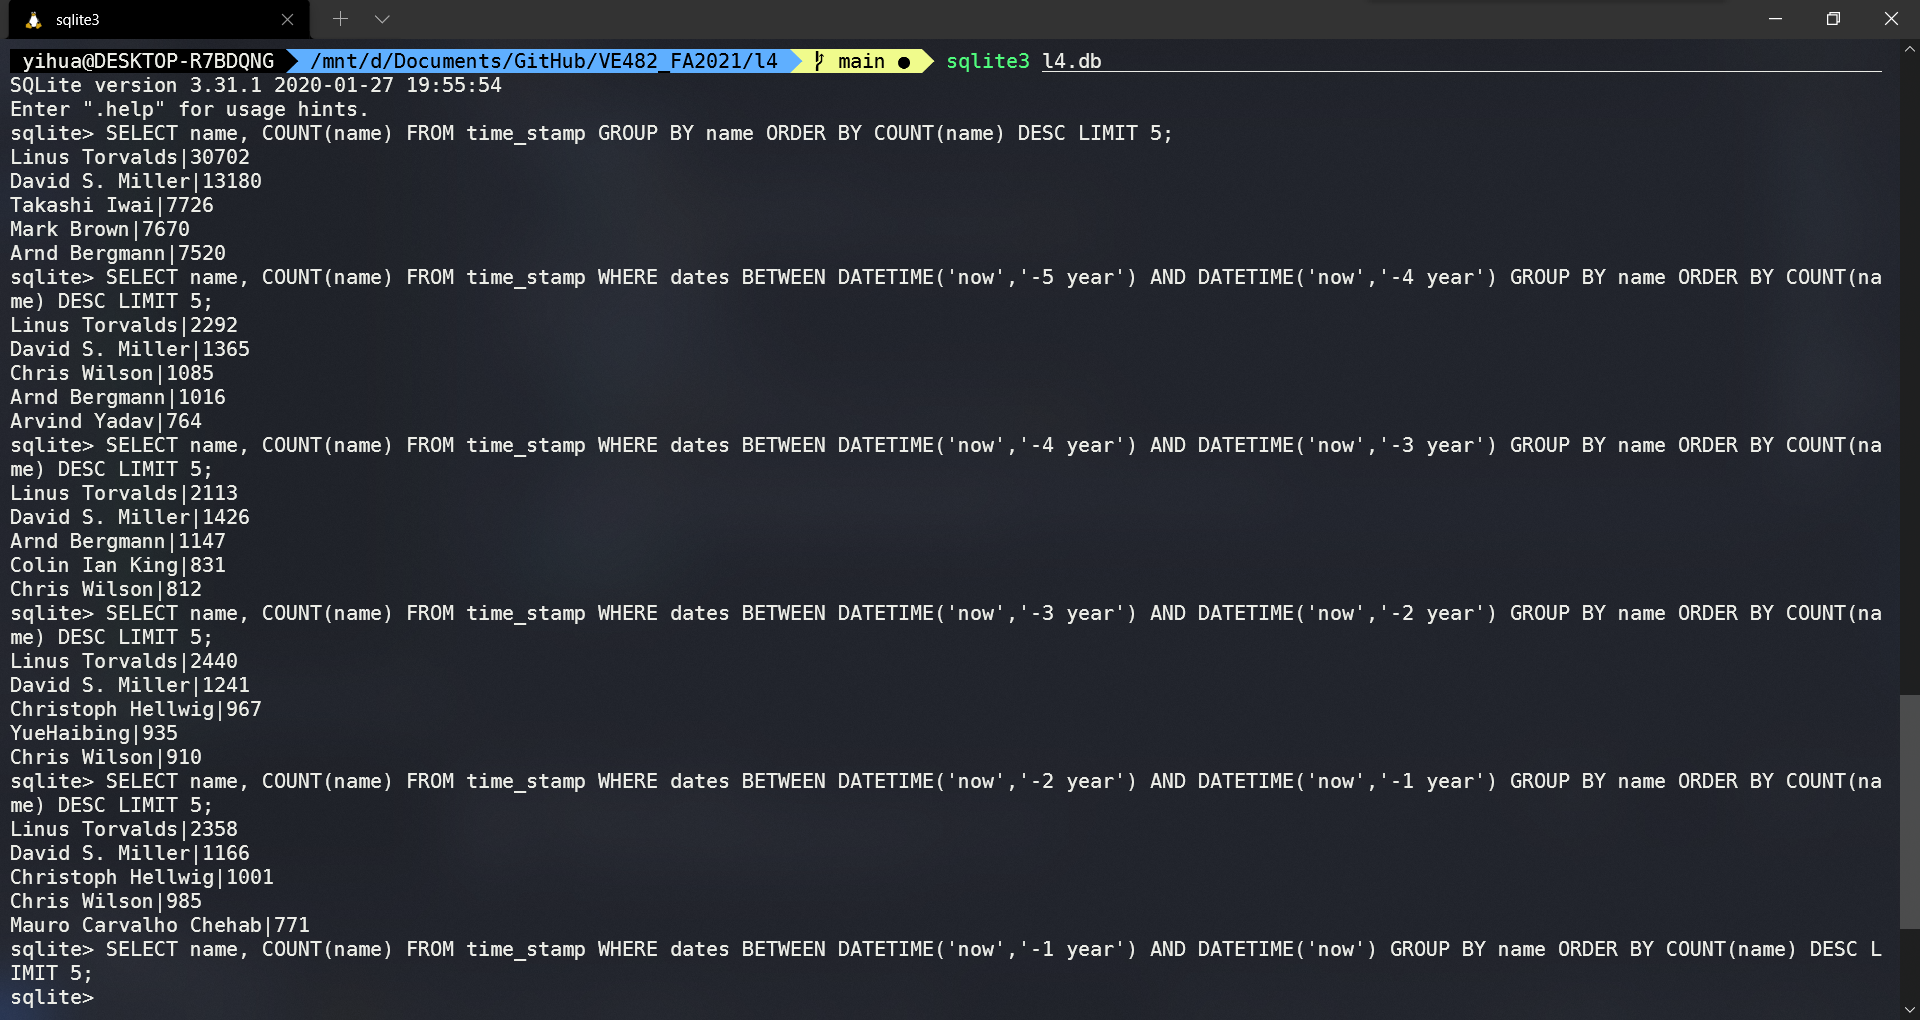
\includegraphics[width=1\textwidth]{8.png}
        \caption{The top five contributors to the Linux kernel since the beginning and each year over the last 5 years.}
    \end{figure}
    \item What is the most common “commit subject”?
    \begin{minted}[frame=single,bgcolor=bg,breaklines]{sql}
SELECT comment, COUNT(comment) FROM db GROUP BY comment ORDER BY COUNT(comment) DESC LIMIT 1;
    \end{minted}
    \begin{minted}[frame=single,bgcolor=bg,breaklines,breakanywhere]{text}
Merge git://git.kernel.org/pub/scm/linux/kernel/git/davem/net|670
    \end{minted}
    \item On which day is the number of commits the highest?
    \begin{minted}[frame=single,bgcolor=bg,breaklines]{sql}
SELECT DATE(dates), count(DATE(dates)) FROM time_stamp GROUP BY DATE(dates) ORDER BY count(DATE(dates)) DESC LIMIT 5;
    \end{minted}
    \begin{minted}[frame=single,bgcolor=bg,breaklines]{text}
2008-01-30|1031
    \end{minted}
    \item Determine the average time between two commits for the five main contributor.
    \begin{minted}[frame=single,bgcolor=bg,breaklines]{sql}
SELECT (MAX(tstamp) - MIN(tstamp)) / (COUNT(DISTINCT(tstamp)) - 1) FROM time_stamp WHERE name = 'Linus Torvalds';
SELECT (MAX(tstamp) - MIN(tstamp)) / (COUNT(DISTINCT(tstamp)) - 1) FROM time_stamp WHERE name = 'David S. Miller';
SELECT (MAX(tstamp) - MIN(tstamp)) / (COUNT(DISTINCT(tstamp)) - 1) FROM time_stamp WHERE name = 'Takashi Iwai';
SELECT (MAX(tstamp) - MIN(tstamp)) / (COUNT(DISTINCT(tstamp)) - 1) FROM time_stamp WHERE name = 'Mark Brown';
SELECT (MAX(tstamp) - MIN(tstamp)) / (COUNT(DISTINCT(tstamp)) - 1) FROM time_stamp WHERE name = 'Arnd Bergmann';
    \end{minted}
    \begin{minted}[frame=single,bgcolor=bg,breaklines]{text}
15886
36972
63730
63205
64693
    \end{minted}
    \begin{figure}[H]
        \centering
        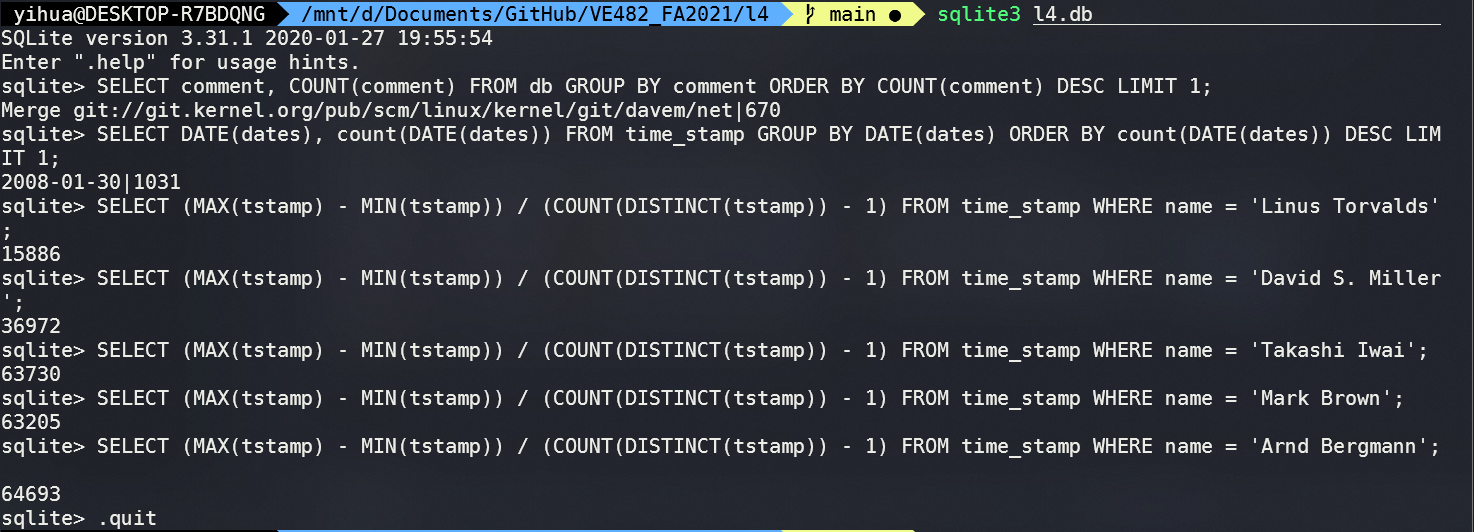
\includegraphics[width=1\textwidth]{9.png}
        \caption{The results of the last three questions.}
    \end{figure}
    The time differences are measured in seconds. Note that Microsoft Access does not support syntax \texttt{COUNT(DISTINCT \textit{column\_name})}. In MySQL, you can use function \texttt{TIMESTAMPDIFF()} to calculate them more flexibly \cite{tstampdiff}.
\end{itemize}
\section{Debugging}
You are pretty happy and enjoying the database tasks when your mum pops in your room. She looks pretty upset that you are still not asleep as she thinks you were playing video games…

When you explain her to that you have terrible bugs in your shell and needed a bit of change, she asked you whether you had used GDB. As you replied “Can I eat it?” she realises you probably do not know much about it. She kindly tells you to have a quick try at it on your current \texttt{mumsh} version to preview it. This should become very handy if you ever have to work on a large scale project.
\begin{itemize}
    \item How to enable built-in debugging in \texttt{gcc}?\\
    Adding a \texttt{-g} option. It can produce debugging information in the operating system’s native format (stabs, COFF, XCOFF, or DWARF). GDB can work with this debugging information \cite{gcc}.
    \item What is the meaning of GDB?\\
    GDB is the GNU Project debugger that allows you to see what is going on `inside' another program while it executes -- or what another program was doing at the moment it crashed, and can do four main kinds of things (plus other things in support of these) to help you catch bugs \cite{gdb}.
    \item Compile the master branch of your \texttt{mumsh} with debugging enabled.
    \begin{minted}[frame=single,bgcolor=bg,breaklines]{bash}
gcc -std=gnu11 -O2 -Wall -Wextra -Werror -pedantic -Wno-unused-result -Wconversion -fno-omit-frame-pointer -fsanitize=undefined -fsanitize=address -o mumsh p1.c -g
    \end{minted}
\end{itemize}
\subsection{Basic GDB usage}
\begin{itemize}
    \item Find the homepage of the GDB project \cite{gdb}.\\
    https://www.gnu.org/software/gdb
    \item What languages are supported by GDB?\\
    GDB supports the following languages (in alphabetical order) \cite{gdb}:
    \begin{itemize}
        \item Ada
        \item Assembly
        \item C
        \item C++
        \item D
        \item Fortran
        \item Go
        \item Objective-C
        \item OpenCL
        \item Modula-2
        \item Pascal
        \item Rust
    \end{itemize}
    \begin{minted}[frame=single,bgcolor=bg,breaklines]{text}
(gdb) file mumsh
(gdb) break p1.c:17
(gdb) break strqtok
(gdb) run
mumsh $ echo 123
(gdb) next
(gdb) step
(gdb) watch delim_offset
(gdb) print delim_offset
(gdb) 
(gdb) continue
(gdb) continue
(gdb) continue
mumsh $ exit
(gdb) continue
(gdb) continue
    \end{minted}
    \begin{figure}[H]
        \centering
        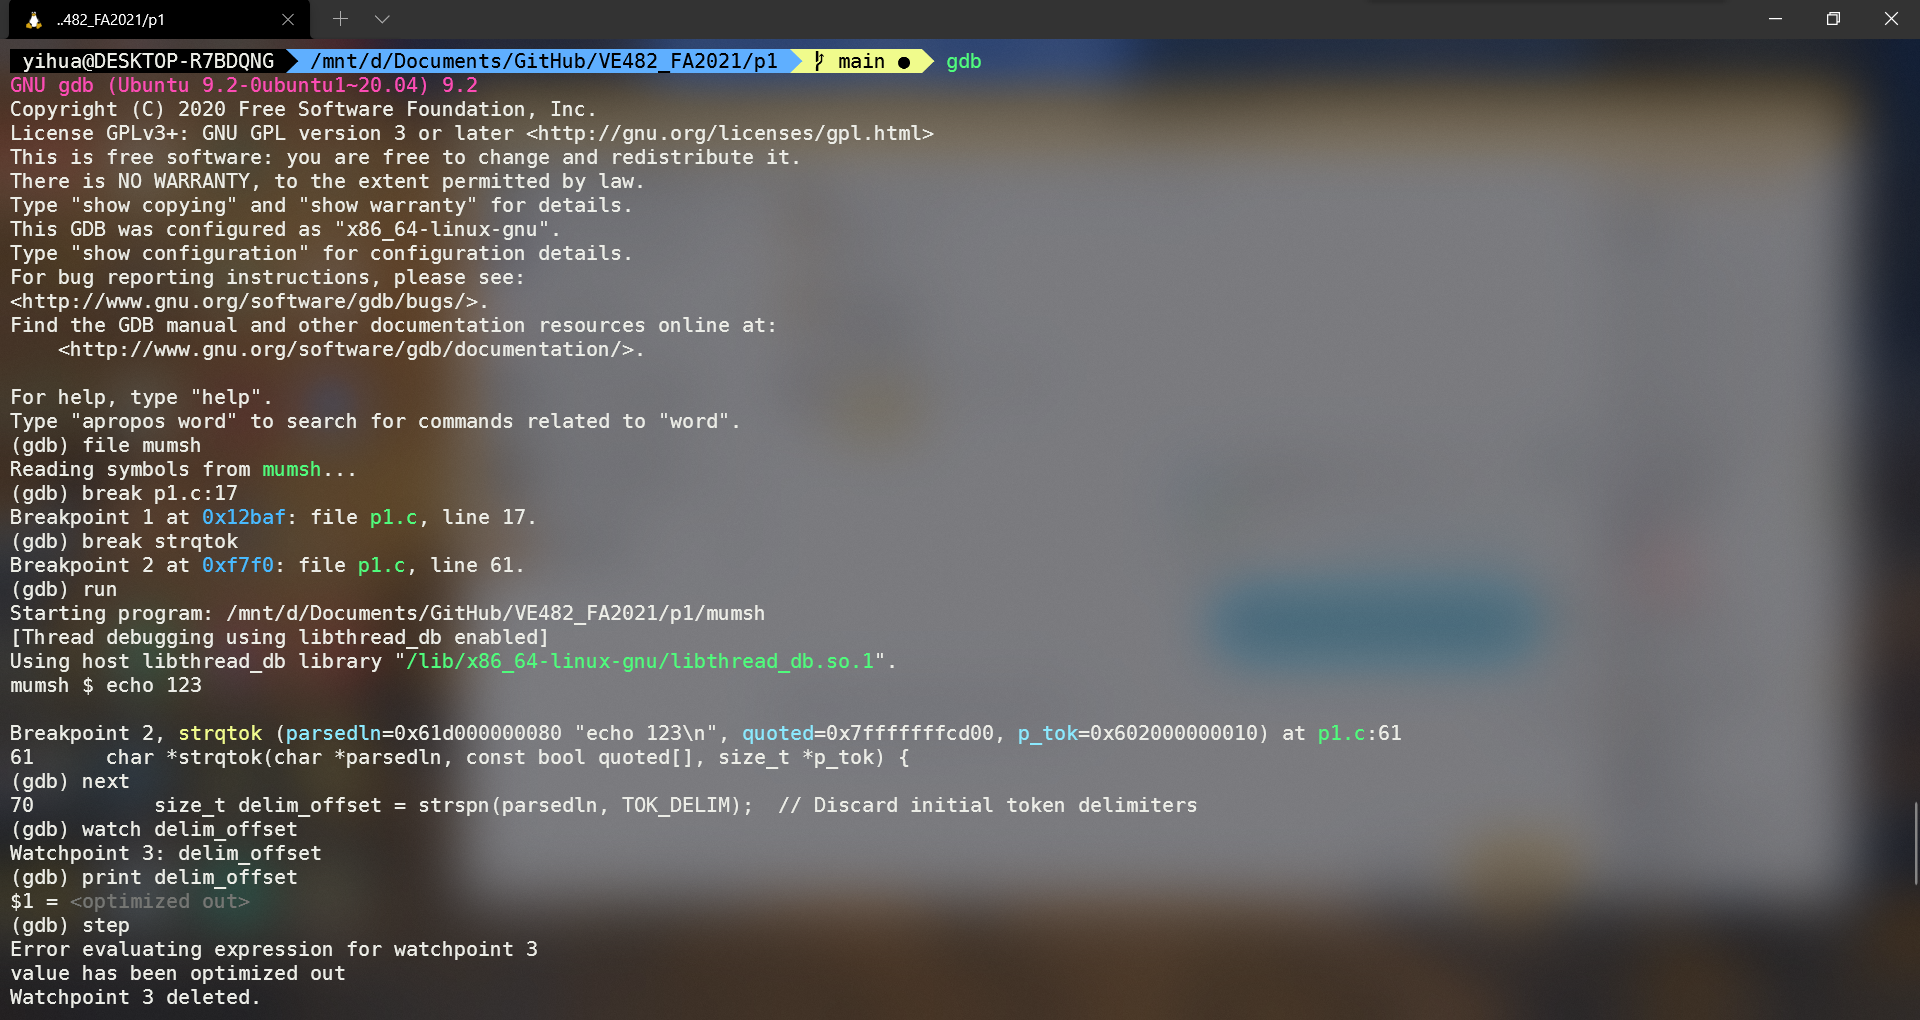
\includegraphics[width=1\textwidth]{10.png}
        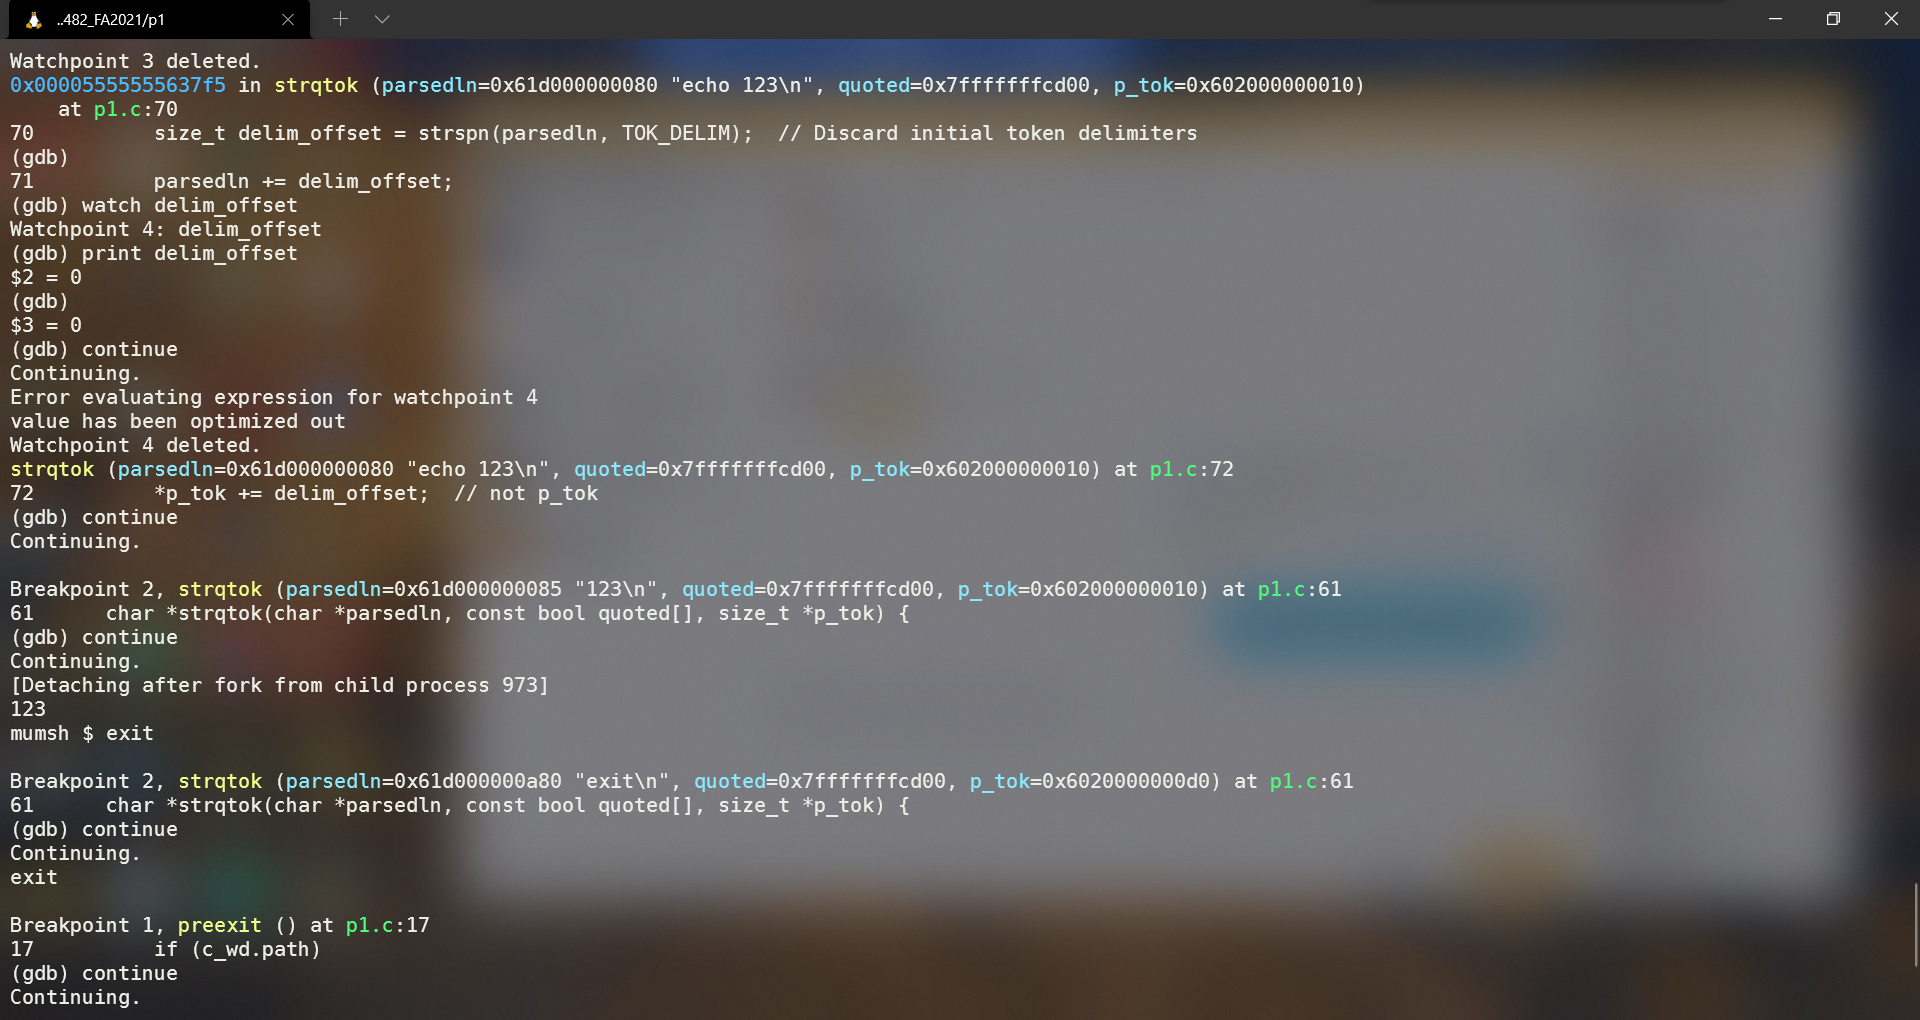
\includegraphics[width=1\textwidth]{11.png}
        \caption{Working with GDB.}
    \end{figure}
    \item What are the following GDB commands doing \cite{gdbum}:
    \begin{itemize}
        \item \texttt{backtrace}: (also \texttt{bt}) A backtrace is a summary of how your program got where it is. It shows one line per frame, for many frames, starting with the currently executing frame (frame zero), followed by its caller (frame one), and on up the stack \cite{backtrace}.
        \item \texttt{delete}: \texttt{delete checkpoint \textit{checkpoint-id}}: Delete the previously-saved checkpoint identified by \textit{checkpoint-id}.\\
        \texttt{delete [breakpoints] [\textit{list...}]}: Delete the breakpoints, watchpoints, or catchpoints of the breakpoint list specified as argument.\\
        \texttt{delete display \textit{dnums...}}: Remove items from the list of expressions to display.\\
        \texttt{delete mem \textit{nums...}}: Remove memory regions \textit{nums}... from the list of regions monitored by gdb.\\
        \texttt{delete tracepoint [\textit{nums...}]}: Permanently delete one or more tracepoints.\\
        \texttt{delete tvariable [\textit{\$name...}]}: Delete the given trace state variables, or all of them if no arguments are specified.
        \item \texttt{where}: The name \texttt{where} is additional alias for \texttt{backtrace}.
        \item \texttt{info breakpoints}: (also \texttt{info break}) Print a table of all breakpoints, watchpoints, and catchpoints set and not deleted.
        \item \texttt{finish}: (also \texttt{fin}) Continue running until just after function in the selected stack frame returns. Print the returned value (if any).
    \end{itemize}
    \item Search the documentation and explain how to use conditional breakpoints \cite{gdbum}.\\
    A breakpoint with a condition evaluates the expression each time your program reaches it, and your program stops only if the condition is \texttt{true}.\\
    \texttt{condition \textit{bnum expression}}: Specify expression as the break condition for breakpoint, watchpoint, or catchpoint number \textit{bnum}.\\
    \texttt{condition -force \textit{bnum expression}}: When the \texttt{-force} flag is used, define the condition even if \textit{expression} is invalid at all the current locations of breakpoint \textit{bnum}.\\
    \texttt{condition \textit{bnum}}: Remove the condition from breakpoint number \textit{bnum}. It becomes an ordinary unconditional breakpoint.\\
    Watch this \href{https://www.youtube.com/watch?v=PorfLSr3DDI}{youtube} video and answer the following questions.
    \item What is \texttt{-tui} option for GDB?\\
    \texttt{tui reg float}: show floating registers.\\
    The GDB Text User Interface (TUI) is a terminal interface which uses the \texttt{curses} library to show the source file, the assembly output, the program registers and GDB commands in separate text windows \cite{tui}.
    \item What is the “reverse step” in GDB and how to enable it. Provide the key steps and commands.\\
    When a program is executed in reverse, the instructions that have most recently been executed are “un-executed”, in reverse order. The program counter runs backward, following the previous thread of execution in reverse. As each instruction is “un-executed”, the values of memory and/or registers that were changed by that instruction are reverted to their previous states. After executing a piece of source code in reverse, all side effects of that code should be “undone”, and all variables should be returned to their prior values \cite{reverse}.\\
    \texttt{reverse-stepi [\textit{count}]}: Reverse-execute one machine instruction.\\
    \texttt{reverse-continue [\textit{ignore-count}]}: (also \texttt{rc [\textit{ignore-count}]}) Beginning at the point where your program last stopped, start executing in reverse. Reverse execution will stop for breakpoints and synchronous exceptions (signals), just like normal execution.
    \begin{minted}[frame=single,bgcolor=bg,breaklines,linenos]{text}
(gdb) p $pc
(gdb) x 0x5e4c5d00
(gdb) bt
(gdb) reverse-stepi
(gdb) bt
(gdb) disas
(gdb) print $sp
(gdb) print *(long **) 0x7fffffffdc98
(gdb) watch *(long **) 0x7fffffffdc98
(gdb) reverse-continue
    \end{minted}
    Line 4 and Line 10 are key steps and commands.
\end{itemize}
\printbibliography
\end{document}